\section{Serialization}

At the end of the day, any consistent memory model requires some form
of serialization.  Indeed, it is well known that sequential
consistency can be implemented by ensuring that all operations on a
given memory address are totally ordered~\cite{ivy}.  In this section,
we survey the alternatives avaialble in existing RDMA hardware, ranging from optimistic approaches that detect and recover from reordering to those that enforce varying degrees of serialization.

\subsection{Locking overhead}

In principle, clients can deal with potential conflicts by utilizing
the atomic operations provided by the RDMA specification, such as
\texttt{compare-and-swap} (\texttt{c\&s]}).  Like their local CPU
  counterparts, atomic compare-and-swap operations enable (seemingly)
  lock-free updates to far data by detecting races and allowing
  clients to implement recovert mechanisms.  In practice, however,
  these atomics are famously~\cite{herd} expensive, fundamentally
  because they require mutual exclusion across all queue pairs to
  deliver their functionality.

\subsection{Memory management hardware}

Hence, a performant far memory system should avoid the use of atomic
operations if at all possible, relying instead on standard RMDA verbs.
Even in that case, existing hardware does provide some guarantees.  For
example, RDMA provides access to memory hosted on a server that likely
utilizes a commodity hardware memory managment unit (MMU).  All modern
MMUs ensure coherent memory accesses, and generally ensure a total
ordering on local memory requests.  Unfortunately, due to the
complexities of today's multi-core, NUMA backplanes and PCIe bus
arbitartion, it is possible that memory requests may not be serviced
in the order they are dispatched.  Happily, the RDMA specification
requires that NICs enforce ordering accross operations in an
individual queue pair, so sequential consistency can be ensured by
ensuring that all requests for a given memory location arrive on the
same queue pair.



\todo{modify this paragraph so that it is closer to the truth}
Figure~\ref{fig:reorder} shows that this guarantee is actually required: i.e.,
requests across queue pairs are \emph{not} always processed in the order
received in practice.  In this example, we use RDMA \texttt{t\&s} operations to
detect reordering.  Specifically, we generate a sequence of test-and-set
operations that increment the value stored at the indicated location by one if
and only if the current value is as expected, i.e., one lower.  Because we
ensure the operations are delivered to the NIC sequentially, a failed operation
indicates the request was reordered internal to the remote server.  We generate
operations for 1,000 different physical addresses (according to a Zipf
distribution) using a varying number of queue pairs and report the frequency
with which they are reordered with respect to another request for the same
address (i.e., the \texttt{t\&s} operation fails).  As expected, when all
requests are issued on the same queue pair, they are serviced in order.  Once a
non-trivial level of concurrency is reached, however, the reordering becomes
significant, with over 7\% of requests to the same address serviced out of order
when they are spread across 32 queue pairs.\sg{given a zipf distribution, and
16qp around 3% of packets are reordered. This is detected by checking the
sequence numbers against the known monotonic sequence.}

\begin{figure}[t]
    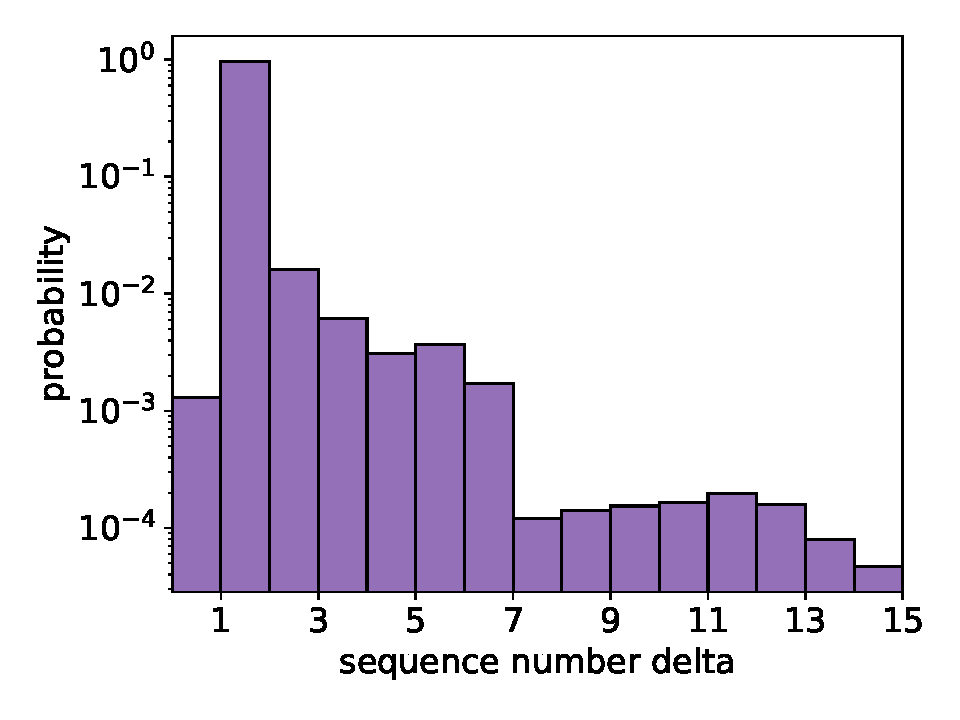
\includegraphics[width=0.45\textwidth]{fig/qp_reordering.pdf}
    \caption{CDF of packet reorderings once QP mapping is applied to a zipf distribution}
    \label{fig:reorder}
\end{figure}

\subsection{Queue pair bottlenecks}

 There are two challenges to restricting requests for a given address
 to a single queue pair---one that can be worked around, and one that
 must be addressed.  First, queue pairs are established on a
 client/server basis, so requests from different clients must arrive
 on differnt queue pairs.  Second, the performance of a single queue
 pair on commercial NICs is significantly less than line rate (likely
 precisely because of the need to enforce ordering constraints).

\begin{figure}[t]
    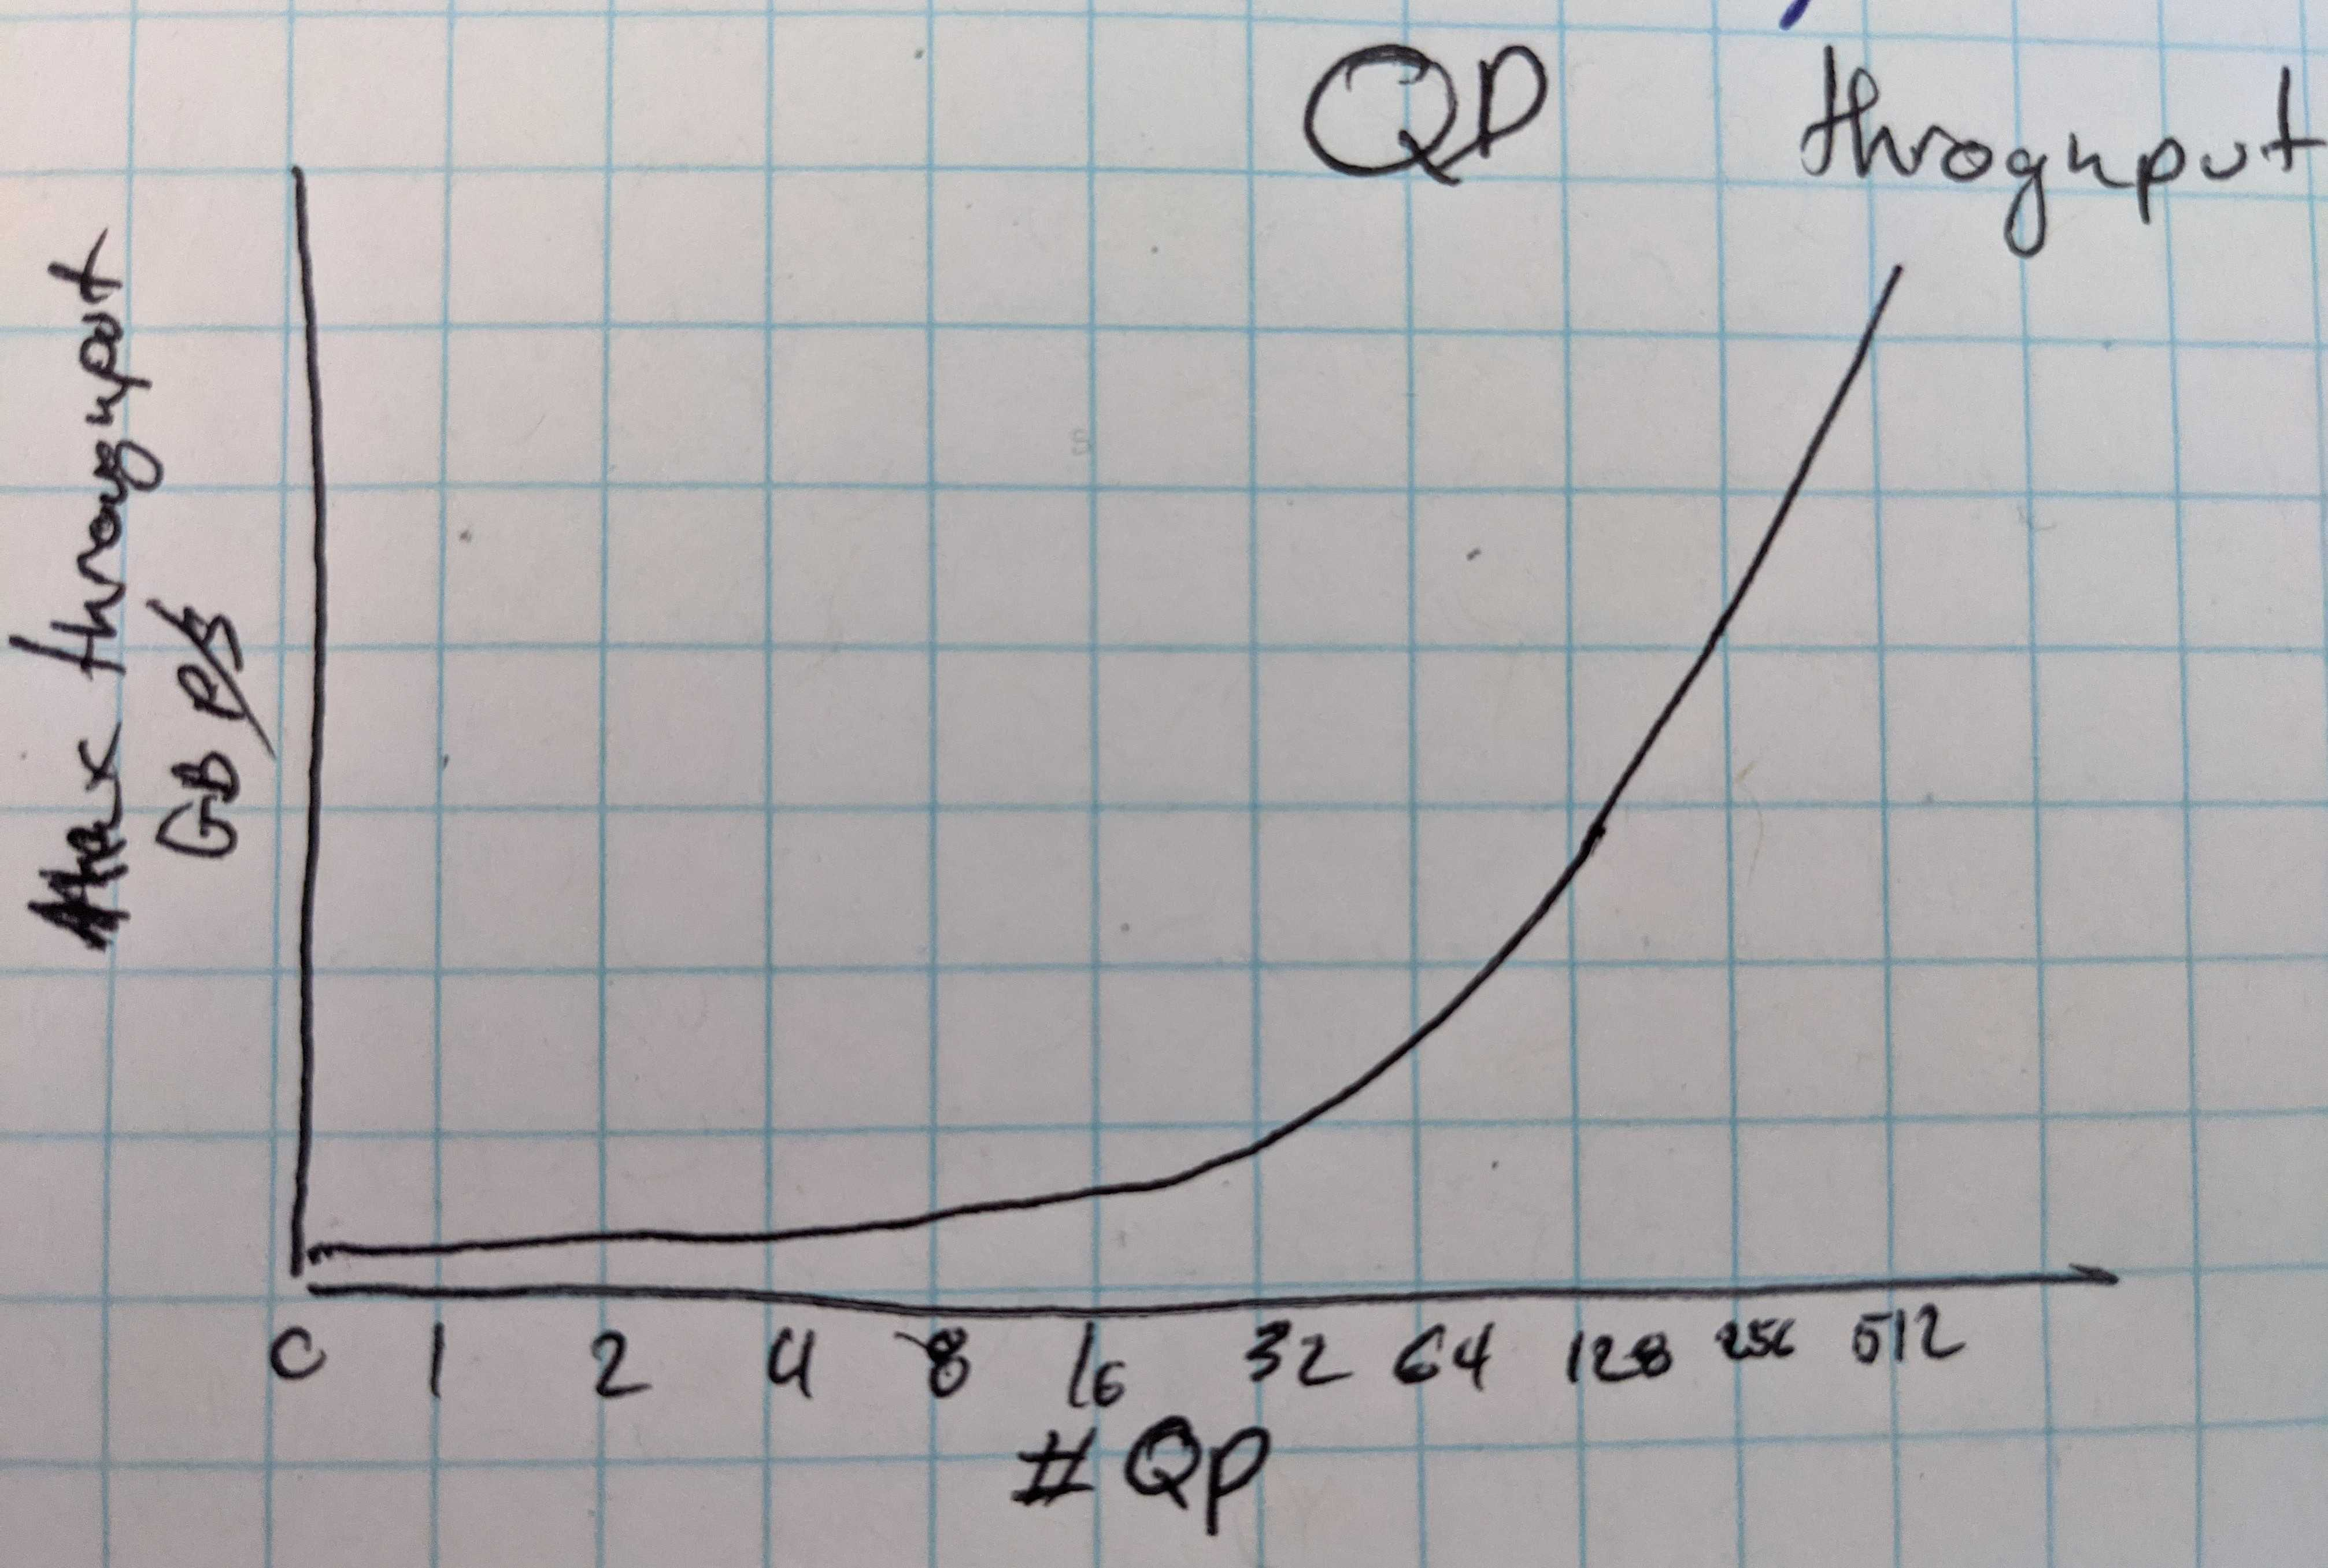
\includegraphics[width=0.45\textwidth]{fig/qp_bottleneck.jpg}
    \caption{Max throughput per QP \todo{take real measurement}}
    \label{fig:qp_bottleneck}
\end{figure}

 





